\documentclass[12pt,halfline,a4paper,]{ouparticle}

% Packages I think are necessary for basic Rmarkdown functionality
\usepackage{hyperref}
\usepackage{graphicx}
\usepackage{listings}
\usepackage{color}
\usepackage{fancyvrb}
\usepackage{framed}

% For knitr::kable functionality
\usepackage{booktabs}
\usepackage{longtable}

%% To allow better options for figure placement
%\usepackage{float}

% Packages that are supposedly required by OUP sty file
\usepackage{amssymb, amsmath, geometry, amsfonts, verbatim, endnotes, setspace}

% For code highlighting I think
\DefineVerbatimEnvironment{Highlighting}{Verbatim}{commandchars=\\\{\}}
\definecolor{shadecolor}{RGB}{248,248,248}
\newenvironment{Shaded}{\begin{snugshade}}{\end{snugshade}}
\newcommand{\AlertTok}[1]{\textcolor[rgb]{0.94,0.16,0.16}{#1}}
\newcommand{\AnnotationTok}[1]{\textcolor[rgb]{0.56,0.35,0.01}{\textbf{\textit{#1}}}}
\newcommand{\AttributeTok}[1]{\textcolor[rgb]{0.77,0.63,0.00}{#1}}
\newcommand{\BaseNTok}[1]{\textcolor[rgb]{0.00,0.00,0.81}{#1}}
\newcommand{\BuiltInTok}[1]{#1}
\newcommand{\CharTok}[1]{\textcolor[rgb]{0.31,0.60,0.02}{#1}}
\newcommand{\CommentTok}[1]{\textcolor[rgb]{0.56,0.35,0.01}{\textit{#1}}}
\newcommand{\CommentVarTok}[1]{\textcolor[rgb]{0.56,0.35,0.01}{\textbf{\textit{#1}}}}
\newcommand{\ConstantTok}[1]{\textcolor[rgb]{0.00,0.00,0.00}{#1}}
\newcommand{\ControlFlowTok}[1]{\textcolor[rgb]{0.13,0.29,0.53}{\textbf{#1}}}
\newcommand{\DataTypeTok}[1]{\textcolor[rgb]{0.13,0.29,0.53}{#1}}
\newcommand{\DecValTok}[1]{\textcolor[rgb]{0.00,0.00,0.81}{#1}}
\newcommand{\DocumentationTok}[1]{\textcolor[rgb]{0.56,0.35,0.01}{\textbf{\textit{#1}}}}
\newcommand{\ErrorTok}[1]{\textcolor[rgb]{0.64,0.00,0.00}{\textbf{#1}}}
\newcommand{\ExtensionTok}[1]{#1}
\newcommand{\FloatTok}[1]{\textcolor[rgb]{0.00,0.00,0.81}{#1}}
\newcommand{\FunctionTok}[1]{\textcolor[rgb]{0.00,0.00,0.00}{#1}}
\newcommand{\ImportTok}[1]{#1}
\newcommand{\InformationTok}[1]{\textcolor[rgb]{0.56,0.35,0.01}{\textbf{\textit{#1}}}}
\newcommand{\KeywordTok}[1]{\textcolor[rgb]{0.13,0.29,0.53}{\textbf{#1}}}
\newcommand{\NormalTok}[1]{#1}
\newcommand{\OperatorTok}[1]{\textcolor[rgb]{0.81,0.36,0.00}{\textbf{#1}}}
\newcommand{\OtherTok}[1]{\textcolor[rgb]{0.56,0.35,0.01}{#1}}
\newcommand{\PreprocessorTok}[1]{\textcolor[rgb]{0.56,0.35,0.01}{\textit{#1}}}
\newcommand{\RegionMarkerTok}[1]{#1}
\newcommand{\SpecialCharTok}[1]{\textcolor[rgb]{0.00,0.00,0.00}{#1}}
\newcommand{\SpecialStringTok}[1]{\textcolor[rgb]{0.31,0.60,0.02}{#1}}
\newcommand{\StringTok}[1]{\textcolor[rgb]{0.31,0.60,0.02}{#1}}
\newcommand{\VariableTok}[1]{\textcolor[rgb]{0.00,0.00,0.00}{#1}}
\newcommand{\VerbatimStringTok}[1]{\textcolor[rgb]{0.31,0.60,0.02}{#1}}
\newcommand{\WarningTok}[1]{\textcolor[rgb]{0.56,0.35,0.01}{\textbf{\textit{#1}}}}

% For making Rmarkdown lists
\providecommand{\tightlist}{%
  \setlength{\itemsep}{0pt}\setlength{\parskip}{0pt}}

% Part for setting citation format package: natbib

% Part for setting citation format package: biblatex

% Part for indenting CSL refs
% Pandoc citation processing
% Pandoc header

\begin{document}

\title{POLS 7012 Final Exam (Answer Key)}

\author{%
\name{YOUR NAME HERE}\address{University of Georgia}\email{\href{mailto:email@email.email}{email@email.email}}
\and
\name{Joseph T. Ornstein}\address{University of Georgia}\email{\href{mailto:jornstein@uga.edu}{jornstein@uga.edu}}
}

\abstract{}

\date{December 09, 2020}

\keywords{}

\maketitle



\hypertarget{introduction}{%
\section{Introduction}\label{introduction}}

In this paper, we will replicate the results from ``Civic Honesty Around
the Globe'' (Cohn et al. 2019). In that paper, the research team dropped
literally thousands of wallets in cities across the globe to see how
many of them get returned. They find, interestingly, that wallets with
money in them are \emph{more} likely to be returned than wallets without
money, which is all very nice and pleasant.

Before you begin, skim over the paper and its Supplementary Materials,
included in the \texttt{papers/} folder. To replicate the findings,
follow the instructions in each section below, writing your code in the
chunks provided. Anything I call an ``extra challenge'' is available to
you if you'd like to give it a try, but is not required. To submit your
final exam, knit this \texttt{.Rmd} to a PDF and post both files
(\texttt{.Rmd} and PDF) to eLC.

\hypertarget{data}{%
\section{Data}\label{data}}

Replication files are available
\href{https://dataverse.harvard.edu/dataverse/honesty}{here}, and I have
taken the liberty of downloading them into the \texttt{data/} folder.
The dataset we'll need for this replication is called the behavioral
data. Let's start by loading it.

\begin{Shaded}
\begin{Highlighting}[]
\NormalTok{data <-}\StringTok{ }\KeywordTok{read_csv}\NormalTok{(}\StringTok{'data/behavioral data (csv file).csv'}\NormalTok{)}
\end{Highlighting}
\end{Shaded}

\hypertarget{results}{%
\section{Results}\label{results}}

\hypertarget{replicating-figure-1}{%
\subsection{Replicating Figure 1}\label{replicating-figure-1}}

Our first task is to replicate the left-hand side of Figure 1. To do so,
we need to perform the following steps:

\begin{itemize}
\tightlist
\item
  Keep only the observations in the Money and NoMoney conditions.
\item
  Recode the \texttt{cond} variable as ``Money'' and ``NoMoney''.
\item
  Compute the average reporting rate, grouped by country and condition.
\item
  Build a scatter plot with average reporting rate on the x-axis,
  country on the y-axis, and colored by monetary condition.
\end{itemize}

\noindent As an extra challenge, you can do any combination of the
following:

\begin{itemize}
\tightlist
\item
  Rearrange the y-axis so that the countries with the lowest reporting
  rate appear at the bottom and those with the highest reporting rate
  appear at the top.
\item
  Include line segments between points as in the original figure
\item
  Use the colors from the original figure
\item
  Use \texttt{geom\_text()} to add floating labels for each country like
  in the original figure. This is an extra, \emph{extra} challenge, but
  man is it satisfying when you get it right!
\end{itemize}

\begin{Shaded}
\begin{Highlighting}[]
\CommentTok{# Here's the basic version}
\NormalTok{fig1 <-}\StringTok{ }\NormalTok{data }\OperatorTok\StringTok{ }
\StringTok{  }\KeywordTok{filter}\NormalTok{(cond }\OperatorTok\StringTok{ }\KeywordTok{c}\NormalTok{(}\DecValTok{0}\NormalTok{,}\DecValTok{1}\NormalTok{)) }\OperatorTok\StringTok{ }
\StringTok{  }\KeywordTok{mutate}\NormalTok{(}\DataTypeTok{cond =} \KeywordTok{case_when}\NormalTok{(cond }\OperatorTok{==}\StringTok{ }\DecValTok{1} \OperatorTok{~}\StringTok{ 'Money'}\NormalTok{, }
\NormalTok{                          cond }\OperatorTok{==}\StringTok{ }\DecValTok{0} \OperatorTok{~}\StringTok{ 'NoMoney'}\NormalTok{)) }\OperatorTok\StringTok{ }
\StringTok{  }\CommentTok{# compute reporting rate by country and monetary condition}
\StringTok{  }\KeywordTok{group_by}\NormalTok{(Country,}
\NormalTok{           cond) }\OperatorTok\StringTok{ }
\StringTok{  }\KeywordTok{summarize}\NormalTok{(}\DataTypeTok{pct_reported =} \KeywordTok{mean}\NormalTok{(response)) }\OperatorTok
\StringTok{  }\CommentTok{# plot}
\StringTok{  }\KeywordTok{ggplot}\NormalTok{() }\OperatorTok{+}
\StringTok{  }\KeywordTok{geom_point}\NormalTok{(}\KeywordTok{aes}\NormalTok{(}\DataTypeTok{x=}\NormalTok{pct_reported, }\DataTypeTok{y=}\NormalTok{Country, }\DataTypeTok{color =} \KeywordTok{factor}\NormalTok{(cond))) }\OperatorTok{+}
\StringTok{  }\KeywordTok{labs}\NormalTok{(}\DataTypeTok{x =} \StringTok{'Reporting rate (%)'}\NormalTok{, }\DataTypeTok{y =} \StringTok{''}\NormalTok{, }\DataTypeTok{color =} \StringTok{'Condition'}\NormalTok{) }\OperatorTok{+}
\StringTok{  }\KeywordTok{theme_minimal}\NormalTok{()}

\NormalTok{fig1}
\end{Highlighting}
\end{Shaded}

\begin{figure}[p]
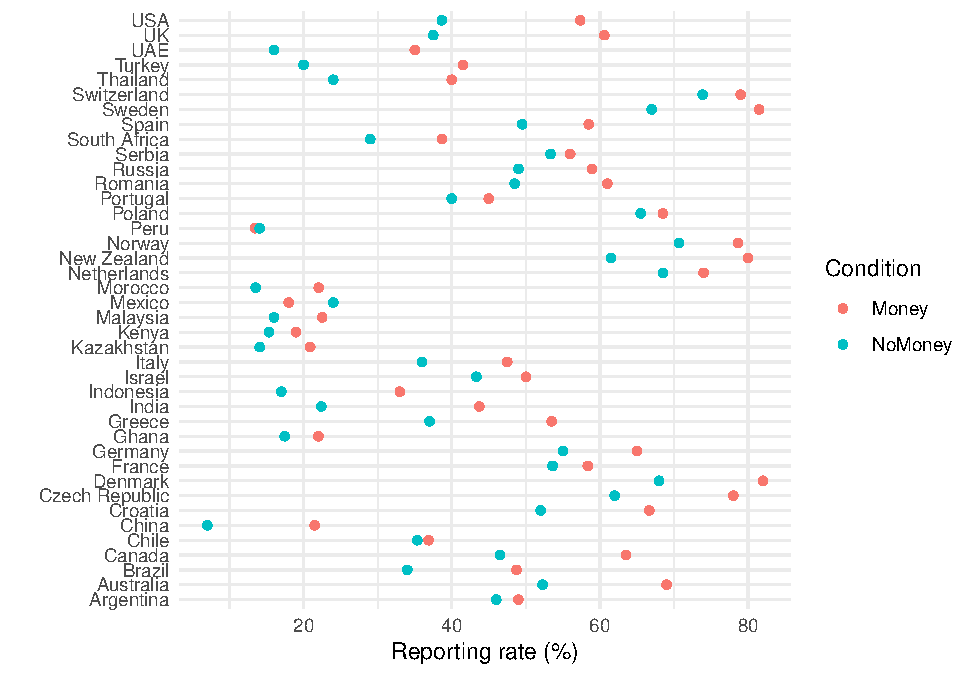
\includegraphics[width=1\linewidth]{final-exam-answer-key_files/figure-latex/Figure 1-1} \caption{Share of wallets reported in the NoMoney and Money conditions, by country.}\label{fig:Figure 1-1}
\end{figure}

\begin{Shaded}
\begin{Highlighting}[]
\CommentTok{# Here's the challenging version}
\NormalTok{fig1a <-}\StringTok{ }\NormalTok{data }\OperatorTok\StringTok{ }
\StringTok{  }\KeywordTok{filter}\NormalTok{(cond }\OperatorTok\StringTok{ }\KeywordTok{c}\NormalTok{(}\DecValTok{0}\NormalTok{,}\DecValTok{1}\NormalTok{)) }\OperatorTok\StringTok{ }
\StringTok{  }\KeywordTok{mutate}\NormalTok{(}\DataTypeTok{cond =} \KeywordTok{case_when}\NormalTok{(cond }\OperatorTok{==}\StringTok{ }\DecValTok{1} \OperatorTok{~}\StringTok{ 'Money'}\NormalTok{, }
\NormalTok{                          cond }\OperatorTok{==}\StringTok{ }\DecValTok{0} \OperatorTok{~}\StringTok{ 'NoMoney'}\NormalTok{)) }\OperatorTok\StringTok{ }
\StringTok{  }\CommentTok{# compute reporting rate by country and monetary condition}
\StringTok{  }\KeywordTok{group_by}\NormalTok{(Country,}
\NormalTok{           cond) }\OperatorTok\StringTok{ }
\StringTok{  }\KeywordTok{summarize}\NormalTok{(}\DataTypeTok{pct_reported =} \KeywordTok{mean}\NormalTok{(response)) }\OperatorTok
\StringTok{  }\CommentTok{# pivot_wider to make those line segments}
\StringTok{  }\NormalTok{ungroup }\OperatorTok\StringTok{ }
\StringTok{  }\KeywordTok{pivot_wider}\NormalTok{(}\DataTypeTok{names_from =}\NormalTok{ cond, }\DataTypeTok{values_from =}\NormalTok{ pct_reported) }\OperatorTok\StringTok{ }
\StringTok{  }\CommentTok{# reorder Country by the NoMoney reporting rate }
\StringTok{  }\KeywordTok{mutate}\NormalTok{(}\DataTypeTok{Country =} \KeywordTok{fct_reorder}\NormalTok{(Country, NoMoney)) }\OperatorTok\StringTok{ }
\StringTok{  }\CommentTok{# compute label position, left of the minimum reporting rate}
\StringTok{  }\KeywordTok{mutate}\NormalTok{(}\DataTypeTok{label_position =} \KeywordTok{pmin}\NormalTok{(Money, NoMoney) }\OperatorTok{-}
\StringTok{           }\KeywordTok{nchar}\NormalTok{(}\KeywordTok{as.character}\NormalTok{(Country))}\OperatorTok{/}\FloatTok{3.5} \OperatorTok{-}\StringTok{ }\DecValTok{1}\NormalTok{) }\OperatorTok\StringTok{ }
\StringTok{  }\CommentTok{# begin ggplot}
\StringTok{  }\KeywordTok{ggplot}\NormalTok{() }\OperatorTok{+}
\StringTok{  }\KeywordTok{geom_segment}\NormalTok{(}\KeywordTok{aes}\NormalTok{(}\DataTypeTok{x=}\NormalTok{Money, }\DataTypeTok{xend=}\NormalTok{NoMoney, }\DataTypeTok{y=}\NormalTok{Country, }\DataTypeTok{yend=}\NormalTok{Country),}
               \DataTypeTok{color =} \StringTok{'gray'}\NormalTok{, }\DataTypeTok{size =} \FloatTok{0.5}\NormalTok{) }\OperatorTok{+}\StringTok{ }
\StringTok{  }\KeywordTok{geom_point}\NormalTok{(}\KeywordTok{aes}\NormalTok{(}\DataTypeTok{x=}\NormalTok{Money,}\DataTypeTok{y=}\NormalTok{Country), }\DataTypeTok{color =} \StringTok{'red'}\NormalTok{) }\OperatorTok{+}
\StringTok{  }\KeywordTok{geom_point}\NormalTok{(}\KeywordTok{aes}\NormalTok{(}\DataTypeTok{x=}\NormalTok{NoMoney,}\DataTypeTok{y=}\NormalTok{Country), }\DataTypeTok{color =} \StringTok{'#F6BE00'}\NormalTok{) }\OperatorTok{+}
\StringTok{  }\KeywordTok{geom_text}\NormalTok{(}\KeywordTok{aes}\NormalTok{(}\DataTypeTok{x=}\NormalTok{label_position, }\DataTypeTok{y=}\NormalTok{Country, }\DataTypeTok{label =}\NormalTok{ Country), }\DataTypeTok{size =} \DecValTok{2}\NormalTok{) }\OperatorTok{+}
\StringTok{  }\KeywordTok{labs}\NormalTok{(}\DataTypeTok{x =} \StringTok{'Reporting rate (%)'}\NormalTok{, }\DataTypeTok{y =} \StringTok{''}\NormalTok{, }\DataTypeTok{color =} \StringTok{'Condition'}\NormalTok{) }\OperatorTok{+}
\StringTok{  }\KeywordTok{theme_classic}\NormalTok{() }\OperatorTok{+}
\StringTok{  }\KeywordTok{theme}\NormalTok{(}\DataTypeTok{axis.text.y =} \KeywordTok{element_blank}\NormalTok{(),}
        \DataTypeTok{axis.ticks.y =} \KeywordTok{element_blank}\NormalTok{(),}
        \DataTypeTok{axis.line.y =} \KeywordTok{element_blank}\NormalTok{())}

\NormalTok{fig1a}
\end{Highlighting}
\end{Shaded}

\begin{figure}[p]
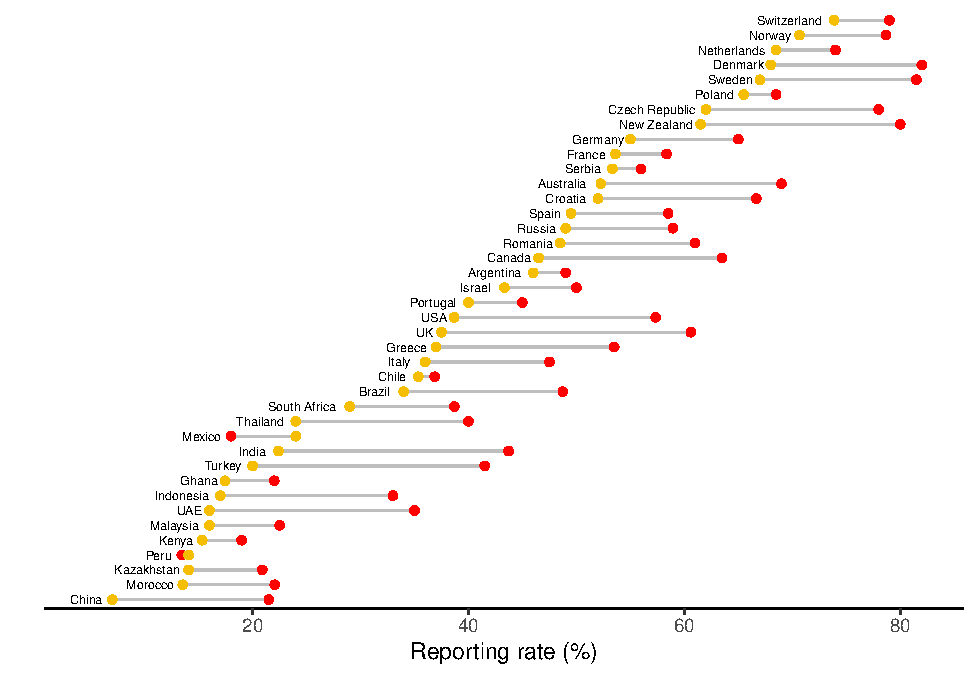
\includegraphics[width=1\linewidth]{final-exam-answer-key_files/figure-latex/Figure 1-2} \caption{Share of wallets reported in the NoMoney and Money conditions, by country.}\label{fig:Figure 1-2}
\end{figure}

\hypertarget{replicating-figure-2}{%
\subsection{Replicating Figure 2}\label{replicating-figure-2}}

Now replicate Figure 2. To do so, we need to perform the following
steps:

\begin{itemize}
\tightlist
\item
  Keep only the data from Poland, the United Kingdom, and the United
  States
\item
  Keep only the NoMoney, Money, and BigMoney conditions
\item
  Recode the \texttt{cond} variable as ``NoMoney'', ``Money'' and
  ``BigMoney''
\item
  Compute the average response rate, grouped by country and condition.
\item
  Plot a scatter with condition on the x-axis, reporting rate on the
  y-axis, and colored by country.
\item
  Add a \texttt{geom\_line()} layer with the same aesthetics (also
  include \texttt{group\ =\ Country} as an aesthetic).
\end{itemize}

\noindent As an extra challenge, you can do any combination of the
following:

\begin{itemize}
\tightlist
\item
  Use original colors from the paper
\item
  Use the ggplot theme that best matches the theme from the paper
\item
  Reorder the \texttt{cond} variable so it appears in the same order as
  the original Figure 2
\item
  Include country labels as in the paper with \texttt{geom\_dl()} from
  the \texttt{directlabels} package, and remove the legend
\end{itemize}

\begin{Shaded}
\begin{Highlighting}[]
\CommentTok{# Basic version}
\NormalTok{data }\OperatorTok\StringTok{ }
\StringTok{  }\KeywordTok{filter}\NormalTok{(Country }\OperatorTok\StringTok{ }\KeywordTok{c}\NormalTok{(}\StringTok{'Poland'}\NormalTok{, }\StringTok{'UK'}\NormalTok{, }\StringTok{'USA'}\NormalTok{),}
\NormalTok{         cond }\OperatorTok\StringTok{ }\DecValTok{0}\OperatorTok{:}\DecValTok{2}\NormalTok{) }\OperatorTok\StringTok{ }
\StringTok{  }\KeywordTok{mutate}\NormalTok{(}\DataTypeTok{cond =} \KeywordTok{case_when}\NormalTok{(cond }\OperatorTok{==}\StringTok{ }\DecValTok{0} \OperatorTok{~}\StringTok{ 'NoMoney'}\NormalTok{,}
\NormalTok{                          cond }\OperatorTok{==}\StringTok{ }\DecValTok{1} \OperatorTok{~}\StringTok{ 'Money'}\NormalTok{,}
\NormalTok{                          cond }\OperatorTok{==}\StringTok{ }\DecValTok{2} \OperatorTok{~}\StringTok{ 'BigMoney'}\NormalTok{)) }\OperatorTok\StringTok{ }
\StringTok{  }\KeywordTok{group_by}\NormalTok{(Country, cond) }\OperatorTok\StringTok{ }
\StringTok{  }\KeywordTok{summarize}\NormalTok{(}\DataTypeTok{reporting_rate =} \KeywordTok{mean}\NormalTok{(response)) }\OperatorTok\StringTok{ }
\StringTok{  }\KeywordTok{ggplot}\NormalTok{() }\OperatorTok{+}\StringTok{ }
\StringTok{  }\KeywordTok{geom_point}\NormalTok{(}\DataTypeTok{mapping =} \KeywordTok{aes}\NormalTok{(}\DataTypeTok{x =}\NormalTok{ cond, }\DataTypeTok{y =}\NormalTok{ reporting_rate,}
                           \DataTypeTok{color =}\NormalTok{ Country)) }\OperatorTok{+}\StringTok{ }
\StringTok{  }\KeywordTok{geom_line}\NormalTok{(}\DataTypeTok{mapping =} \KeywordTok{aes}\NormalTok{(}\DataTypeTok{x =}\NormalTok{ cond, }\DataTypeTok{y =}\NormalTok{ reporting_rate,}
                          \DataTypeTok{group =}\NormalTok{ Country, }\DataTypeTok{color =}\NormalTok{ Country)) }\OperatorTok{+}\StringTok{ }
\StringTok{  }\KeywordTok{labs}\NormalTok{(}\DataTypeTok{x =} \StringTok{''}\NormalTok{, }\DataTypeTok{y =} \StringTok{'Reporting Rate (%)'}\NormalTok{)}
\end{Highlighting}
\end{Shaded}

\begin{figure}[p]
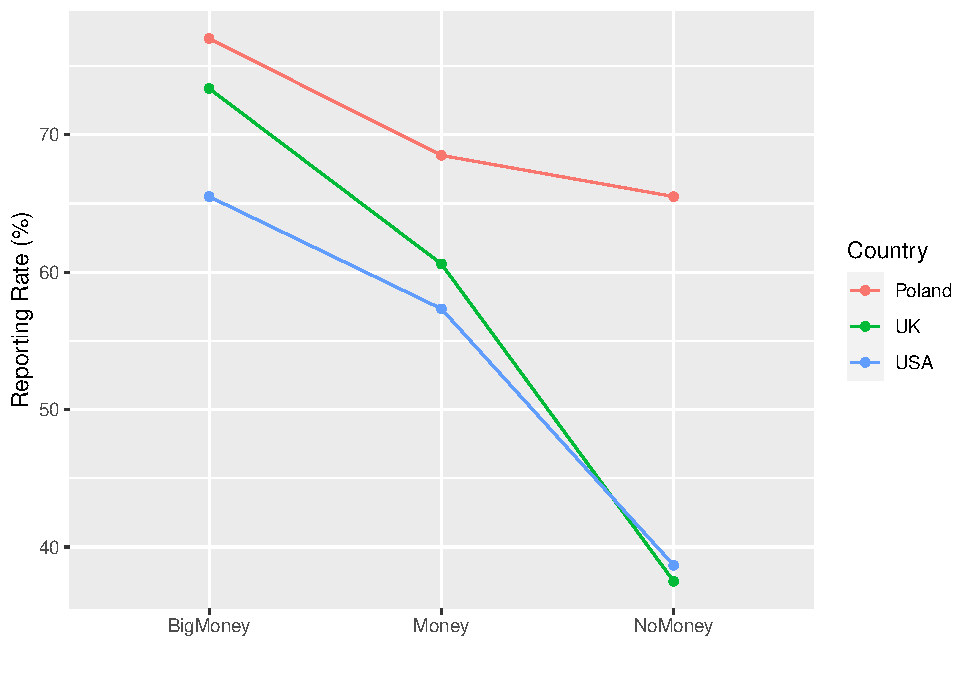
\includegraphics[width=1\linewidth]{final-exam-answer-key_files/figure-latex/Figure 2-1} \caption{Reporting rates as a function of monetary stakes}\label{fig:Figure 2-1}
\end{figure}

\begin{Shaded}
\begin{Highlighting}[]
\KeywordTok{library}\NormalTok{(directlabels)}

\CommentTok{# Harder version}
\NormalTok{data }\OperatorTok\StringTok{ }
\StringTok{  }\KeywordTok{filter}\NormalTok{(Country }\OperatorTok\StringTok{ }\KeywordTok{c}\NormalTok{(}\StringTok{'Poland'}\NormalTok{, }\StringTok{'UK'}\NormalTok{, }\StringTok{'USA'}\NormalTok{),}
\NormalTok{         cond }\OperatorTok\StringTok{ }\DecValTok{0}\OperatorTok{:}\DecValTok{2}\NormalTok{) }\OperatorTok\StringTok{ }
\StringTok{  }\KeywordTok{mutate}\NormalTok{(}\DataTypeTok{Country =} \KeywordTok{case_when}\NormalTok{(Country }\OperatorTok{==}\StringTok{ 'UK'} \OperatorTok{~}\StringTok{ 'United Kingdom'}\NormalTok{,}
\NormalTok{                             Country }\OperatorTok{==}\StringTok{ 'USA'} \OperatorTok{~}\StringTok{ 'United States'}\NormalTok{,}
                             \OtherTok{TRUE} \OperatorTok{~}\StringTok{ }\NormalTok{Country),}
         \DataTypeTok{cond =} \KeywordTok{case_when}\NormalTok{(cond }\OperatorTok{==}\StringTok{ }\DecValTok{0} \OperatorTok{~}\StringTok{ 'NoMoney'}\NormalTok{,}
\NormalTok{                          cond }\OperatorTok{==}\StringTok{ }\DecValTok{1} \OperatorTok{~}\StringTok{ 'Money'}\NormalTok{,}
\NormalTok{                          cond }\OperatorTok{==}\StringTok{ }\DecValTok{2} \OperatorTok{~}\StringTok{ 'BigMoney'}\NormalTok{)) }\OperatorTok\StringTok{ }
\StringTok{  }\KeywordTok{group_by}\NormalTok{(Country, cond) }\OperatorTok\StringTok{ }
\StringTok{  }\KeywordTok{summarize}\NormalTok{(}\DataTypeTok{reporting_rate =} \KeywordTok{mean}\NormalTok{(response)) }\OperatorTok\StringTok{ }
\StringTok{  }\KeywordTok{mutate}\NormalTok{(}\DataTypeTok{cond =} \KeywordTok{factor}\NormalTok{(cond, }\DataTypeTok{levels =} \KeywordTok{c}\NormalTok{(}\StringTok{'NoMoney'}\NormalTok{, }\StringTok{'Money'}\NormalTok{, }\StringTok{'BigMoney'}\NormalTok{))) }\OperatorTok\StringTok{ }
\StringTok{  }\KeywordTok{ggplot}\NormalTok{() }\OperatorTok{+}\StringTok{ }
\StringTok{  }\KeywordTok{geom_point}\NormalTok{(}\DataTypeTok{mapping =} \KeywordTok{aes}\NormalTok{(}\DataTypeTok{x =}\NormalTok{ cond, }\DataTypeTok{y =}\NormalTok{ reporting_rate,}
                           \DataTypeTok{color =}\NormalTok{ Country)) }\OperatorTok{+}\StringTok{ }
\StringTok{  }\KeywordTok{geom_line}\NormalTok{(}\DataTypeTok{mapping =} \KeywordTok{aes}\NormalTok{(}\DataTypeTok{x =}\NormalTok{ cond, }\DataTypeTok{y =}\NormalTok{ reporting_rate,}
                          \DataTypeTok{group =}\NormalTok{ Country, }\DataTypeTok{color =}\NormalTok{ Country)) }\OperatorTok{+}\StringTok{ }
\StringTok{  }\KeywordTok{geom_dl}\NormalTok{(}\DataTypeTok{mapping =} \KeywordTok{aes}\NormalTok{(}\DataTypeTok{x=}\NormalTok{cond, }\DataTypeTok{y=}\NormalTok{reporting_rate, }\DataTypeTok{label =}\NormalTok{ Country),}
          \DataTypeTok{method =} \KeywordTok{list}\NormalTok{(}\KeywordTok{dl.trans}\NormalTok{(}\DataTypeTok{x =}\NormalTok{ x }\OperatorTok{+}\StringTok{ }\FloatTok{0.2}\NormalTok{), }\StringTok{'last.points'}\NormalTok{, }\DataTypeTok{cex =} \FloatTok{0.75}\NormalTok{)) }\OperatorTok{+}
\StringTok{  }\KeywordTok{scale_color_manual}\NormalTok{(}\DataTypeTok{values =} \KeywordTok{c}\NormalTok{(}\StringTok{'#8b1b1e'}\NormalTok{, }\StringTok{'#f23524'}\NormalTok{, }\StringTok{'#f98f1c'}\NormalTok{)) }\OperatorTok{+}
\StringTok{  }\KeywordTok{labs}\NormalTok{(}\DataTypeTok{x =} \StringTok{''}\NormalTok{, }\DataTypeTok{y =} \StringTok{'Reporting Rate (%)'}\NormalTok{) }\OperatorTok{+}
\StringTok{  }\KeywordTok{theme_classic}\NormalTok{() }\OperatorTok{+}
\StringTok{  }\KeywordTok{theme}\NormalTok{(}\DataTypeTok{legend.position =} \StringTok{'none'}\NormalTok{)}
\end{Highlighting}
\end{Shaded}

\begin{figure}[p]
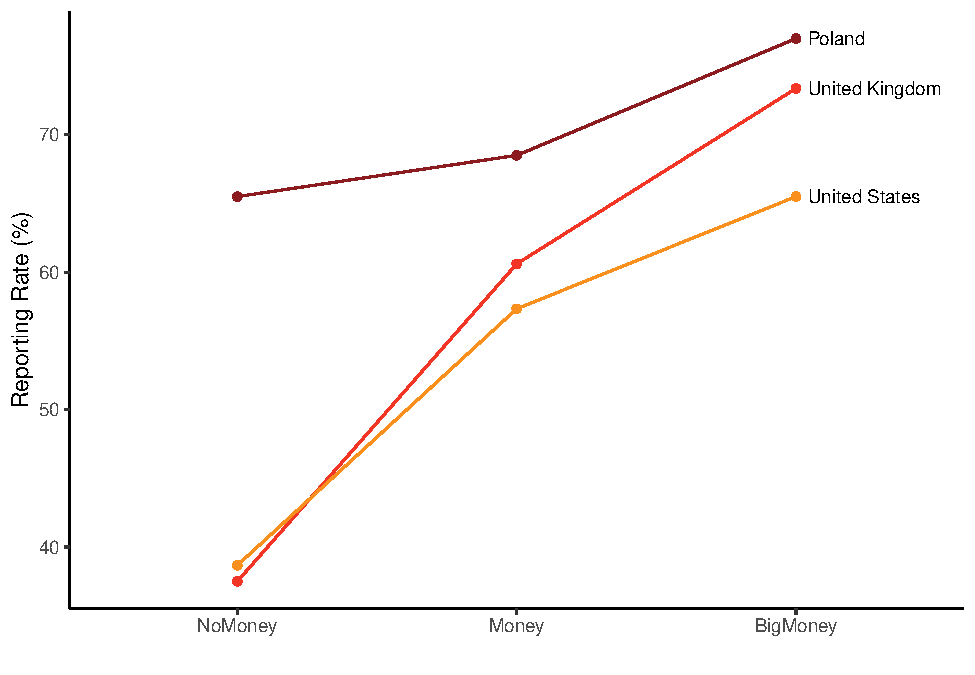
\includegraphics[width=1\linewidth]{final-exam-answer-key_files/figure-latex/Figure 2-2} \caption{Reporting rates as a function of monetary stakes}\label{fig:Figure 2-2}
\end{figure}

\hypertarget{the-effect-of-money}{%
\subsection{The Effect of Money}\label{the-effect-of-money}}

In paragraph 3 of page 2, the authors claim that citizens are
``overwhelmingly more likely to report lost wallets containing money
than those without''. Let's replicate that finding. To do so, we must:

\begin{itemize}
\tightlist
\item
  Keep the observations in the Money and NoMoney conditions
\item
  Compute the percent of subjects that reported wallets without money.
  Save that value, rounded to the nearest percent, as the object
  \texttt{no\_money\_reporting\_rate}.
\item
  Compute the percent of subjects that reported wallets with money. Save
  that value, rounded to the nearest percent, as the object
  \texttt{money\_reporting\_rate}.
\end{itemize}

On average, adding money to the wallet increased the likelihood of being
reported from 40\% in the NoMoney condition to 51\% in the Money
condition.

Next, conduct a hypothesis test to determine the strength of that
result. Our null hypothesis is that there is no difference in reporting
rates between the Money and NoMoney groups. Note that the explanatory
variable (money or no money) and outcome variable (report or not report)
are both categorical. Report the p-value associated with your null
hypothesis test.

\begin{Shaded}
\begin{Highlighting}[]
\NormalTok{data }\OperatorTok\StringTok{ }
\StringTok{  }\KeywordTok{filter}\NormalTok{(cond }\OperatorTok\StringTok{ }\KeywordTok{c}\NormalTok{(}\DecValTok{0}\NormalTok{,}\DecValTok{1}\NormalTok{)) }\OperatorTok\StringTok{ }
\StringTok{  }\KeywordTok{select}\NormalTok{(cond, response) }\OperatorTok\StringTok{ }
\StringTok{  }\NormalTok{table }\OperatorTok\StringTok{ }
\StringTok{  }\KeywordTok{chisq.test}\NormalTok{(}\DataTypeTok{correct =} \OtherTok{FALSE}\NormalTok{)}
\end{Highlighting}
\end{Shaded}

\begin{verbatim}
## 
##  Pearson's Chi-squared test
## 
## data:  .
## X-squared = 201.21, df = 1, p-value < 2.2e-16
\end{verbatim}

\hypertarget{replicating-table-s8}{%
\subsubsection{Replicating Table S8}\label{replicating-table-s8}}

In the Supplementary Materials, the authors extend the bivariate
hypothesis test we just did by estimating two linear models that include
other subject characterstics as covariates. To replicate that finding,
we must:

\begin{itemize}
\tightlist
\item
  Create a variable called \texttt{Money}, equal to 1 if the subject's
  wallet contained money and 0 otherwise.
\item
  Create a variable called \texttt{BigMoney}, equal to 1 if the
  subject's wallet contained \textbf{lots} of money and 0 otherwise.
\item
  Create a variable called \texttt{MoneyNoKey}, equal to 1 if they
  subject's wallet contained money but no key and 0 otherwise.
\item
  To include ``Institution and City Fixed Effects'', make sure that the
  city and type of institution are coded as characters or factors.
\item
  Estimate your first model, \texttt{lm1}, including the treatment
  variables you created plus the institution and city fixed effects.
\item
  In the second model \texttt{lm2}, add the binary variables mentioned
  in the notes of Table S8.
\item
  Don't worry if your standard errors don't exactly match up. You'll
  learn more about ``robust'' standard errors next semester.
\end{itemize}

\begin{Shaded}
\begin{Highlighting}[]
\NormalTok{lm1 <-}\StringTok{ }\KeywordTok{lm}\NormalTok{(response }\OperatorTok{~}\StringTok{ }\NormalTok{male, }\DataTypeTok{data =}\NormalTok{ data)}
\NormalTok{lm2 <-}\StringTok{ }\KeywordTok{lm}\NormalTok{(response }\OperatorTok{~}\StringTok{ }\NormalTok{male, }\DataTypeTok{data =}\NormalTok{ data)}

\NormalTok{data <-}\StringTok{ }\NormalTok{data }\OperatorTok\StringTok{ }
\StringTok{  }\KeywordTok{mutate}\NormalTok{(}\DataTypeTok{Money =} \KeywordTok{if_else}\NormalTok{(cond }\OperatorTok{==}\StringTok{ }\DecValTok{1}\NormalTok{, }\DecValTok{1}\NormalTok{, }\DecValTok{0}\NormalTok{),}
         \DataTypeTok{BigMoney =} \KeywordTok{if_else}\NormalTok{(cond }\OperatorTok{==}\StringTok{ }\DecValTok{2}\NormalTok{, }\DecValTok{1}\NormalTok{, }\DecValTok{0}\NormalTok{),}
         \DataTypeTok{MoneyNoKey =} \KeywordTok{if_else}\NormalTok{(cond }\OperatorTok{==}\StringTok{ }\DecValTok{3}\NormalTok{, }\DecValTok{1}\NormalTok{, }\DecValTok{0}\NormalTok{),}
         \DataTypeTok{institution =} \KeywordTok{factor}\NormalTok{(institution),}
         \DataTypeTok{city =} \KeywordTok{factor}\NormalTok{(city))}

\NormalTok{lm1 <-}\StringTok{ }\KeywordTok{lm}\NormalTok{(response }\OperatorTok{~}\StringTok{ }\NormalTok{Money }\OperatorTok{+}\StringTok{ }\NormalTok{BigMoney }\OperatorTok{+}\StringTok{ }\NormalTok{MoneyNoKey }\OperatorTok{+}\StringTok{ }\NormalTok{institution }\OperatorTok{+}\StringTok{ }\NormalTok{city, }\DataTypeTok{data =}\NormalTok{ data)}
\NormalTok{lm2 <-}\StringTok{ }\KeywordTok{lm}\NormalTok{(response }\OperatorTok{~}\StringTok{ }\NormalTok{Money }\OperatorTok{+}\StringTok{ }\NormalTok{BigMoney }\OperatorTok{+}\StringTok{ }\NormalTok{MoneyNoKey }\OperatorTok{+}\StringTok{ }\NormalTok{institution }\OperatorTok{+}\StringTok{ }\NormalTok{city }\OperatorTok{+}
\StringTok{            }\NormalTok{male }\OperatorTok{+}\StringTok{ }\NormalTok{above40 }\OperatorTok{+}\StringTok{ }\NormalTok{computer }\OperatorTok{+}\StringTok{ }\NormalTok{coworkers }\OperatorTok{+}\StringTok{ }\NormalTok{other_bystanders, }\DataTypeTok{data =}\NormalTok{ data)}
\end{Highlighting}
\end{Shaded}

The following code chunk outputs a pretty table like the one in Table
S8. I provide it to you free of charge. All you need to do is make sure
that \texttt{lm1} and \texttt{lm2} are correctly specified.

\begin{table}[!htbp] \centering 
  \caption{Reporting rates in the Money and NoMoney condition} 
  \label{} 
\begin{tabular}{@{\extracolsep{5pt}}lcc} 
\\[-1.8ex]\hline 
\hline \\[-1.8ex] 
\\[-1.8ex] & (1) & (2)\\ 
\hline \\[-1.8ex] 
 Money & 10.828$^{***}$ & 10.791$^{***}$ \\ 
  & (0.716) & (0.713) \\ 
  & & \\ 
 male &  & $-$2.076$^{**}$ \\ 
  &  & (0.740) \\ 
  & & \\ 
 above40 &  & $-$2.030$^{**}$ \\ 
  &  & (0.737) \\ 
  & & \\ 
 computer &  & 6.874$^{***}$ \\ 
  &  & (0.975) \\ 
  & & \\ 
 coworkers &  & 4.675$^{***}$ \\ 
  &  & (0.771) \\ 
  & & \\ 
 other\_bystanders &  & $-$3.900$^{***}$ \\ 
  &  & (0.798) \\ 
  & & \\ 
 Constant & 34.620$^{**}$ & 33.302$^{**}$ \\ 
  & (10.687) & (10.720) \\ 
  & & \\ 
\hline \\[-1.8ex] 
Observations & 17,303 & 17,295 \\ 
Adjusted R$^{2}$ & 0.178 & 0.185 \\ 
\hline 
\hline \\[-1.8ex] 
\textit{Note:}  & \multicolumn{2}{r}{$^{*}$p$<$0.05; $^{**}$p$<$0.01; $^{***}$p$<$0.001} \\ 
\end{tabular} 
\end{table}

\hypertarget{conclusion}{%
\section{Conclusion}\label{conclusion}}

Hey people are more likely to try to return wallets they find if they
have money in them. Isn't that nice?

\hypertarget{references}{%
\section*{References}\label{references}}
\addcontentsline{toc}{section}{References}

\hypertarget{refs}{}
\leavevmode\hypertarget{ref-cohnCivicHonestyGlobe2019}{}%
Cohn, Alain, Michel André Maréchal, David Tannenbaum, and Christian
Lukas Zünd. 2019. ``Civic Honesty Around the Globe.'' \emph{Science} 365
(6448): 70--73. \url{https://doi.org/10.1126/science.aau8712}.






\end{document}
